% =============================================================================
%  APPENDIX: PIPELINE ARCHITECTURE  (backup slide; thesis Figure 4.1)
% =============================================================================
\begin{frame}{Appendix: The Twelve-Stage Pipeline}
\begin{atucols}[c]
\begin{column}{0.42\textwidth}
  \centering
  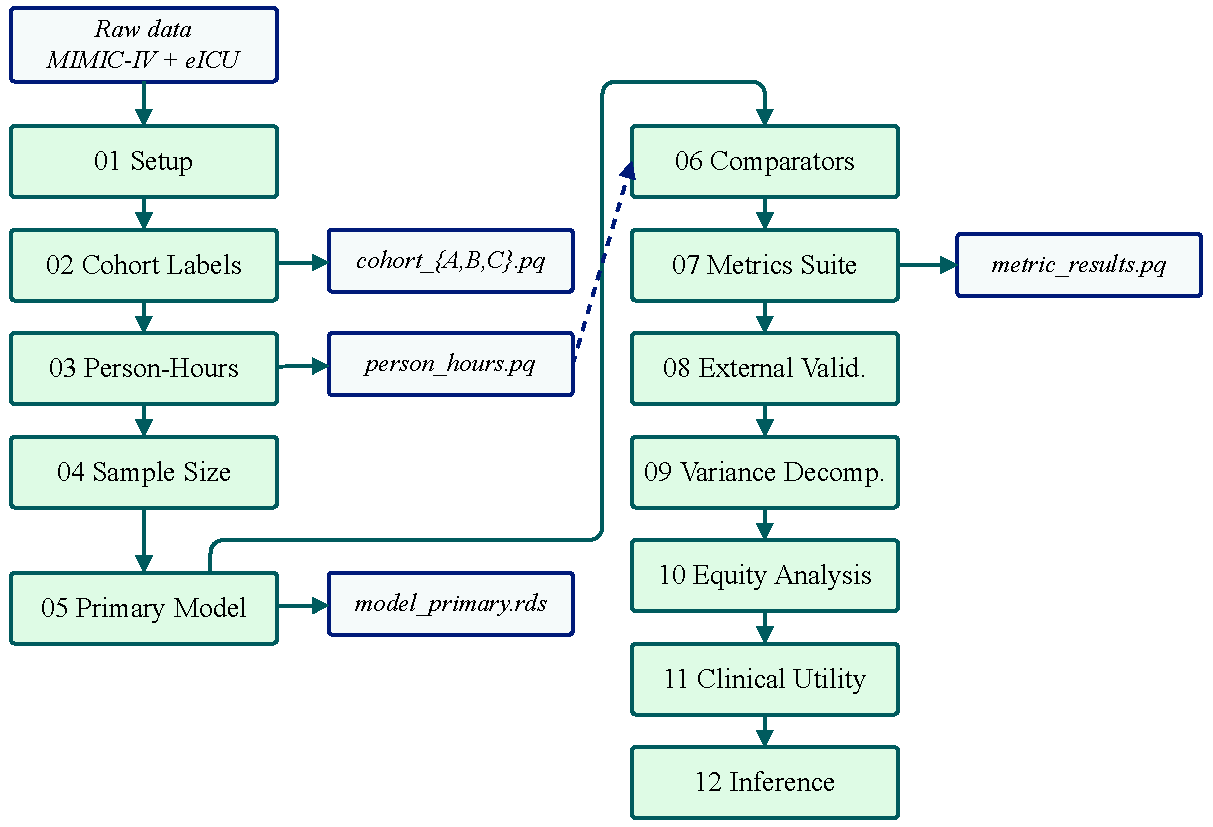
\includegraphics[width=\columnwidth,height=0.76\textheight,
                   keepaspectratio]{images/fig4.1_pipeline_dag.pdf}
\end{column}
\begin{column}{0.56\textwidth}
\begin{itemize}\itemsep3pt\small
  \item One orchestration script runs stages 01--12; a single configuration
        module defines the file paths, identifiers and analytical thresholds.
  \item Reported results are generated directly from the pipeline outputs,
        reducing the risk of transcription errors between analysis and
        thesis.
  \item Frozen-run tag: \texttt{\pcFrozenTag}.
  \item Code and reproducibility:\\ {\scriptsize\repolink}
\end{itemize}
\end{column}
\end{atucols}
\end{frame}
